\documentclass[]{scrartcl}
\usepackage[a4paper,left=2cm,right=3cm,top=2cm,bottom=2cm]{geometry}
\usepackage{svg}
\usepackage{graphicx}
\usepackage[dvipsnames]{xcolor}
\usepackage{minted}
\usepackage{tcolorbox}
\usepackage[spanish]{babel}
\usepackage{mdframed}
\usepackage{epigraph}
\usepackage{wrapfig}


\tcbuselibrary{minted}
\tcbuselibrary{breakable}

\definecolor{bashcodebg}{rgb}{0.85,0.85,0.85}

\newtcolorbox{notebox}{colback=SpringGreen!15!white,
colframe=SpringGreen!50!black}

\newtcolorbox{importantbox}{colback=RubineRed!25!white,colframe=RubineRed!75!black}

\newtcolorbox[auto counter]{exbox}[1][]{%
colback=red!5!white,colframe=red!75!black,
fonttitle=\bfseries,
title=Ejercicio \thetcbcounter: , #1}

\newtcblisting[auto counter]{cbox}[2][]{%
listing engine=minted,
minted language=c,
minted style=friendly,
minted options={mathescape,autogobble, framesep},
colback=TealBlue!5!white,colframe=TealBlue!75!black,
fonttitle=\bfseries,
listing only,
title=Snippet \thetcbcounter: #2, 
nameref=Snippet \thetcbcounter: #2,
#1}

\newminted[ccode]{c}{
  style=friendly,
  linenos=false,
  autogobble,
  fontsize=\footnotesize,
  bgcolor=gray!5,
  framesep=2mm,
  baselinestretch=1.2 % Adjust line height if needed
}

\newtcblisting[auto counter]{bashbox}[1][]{%
listing engine=minted,
minted language=bash,
minted style=friendly,
minted options={mathescape,autogobble, framesep},
colback=bashcodebg,
colframe=black!70,
fonttitle=\bfseries,
listing only,
#1}

\newtcbinputlisting[]{\bashinput}[2][]{%
listing file={#2},
listing engine=minted,
minted language=bash,
minted style=friendly,
minted options={autogobble, framesep},
colback=bashcodebg,
colframe=black!70,
fonttitle=\bfseries,
listing only,
#1}

\usepackage{colortbl} % para /color
\usepackage{hyperref} % Necesario para \url y \href
\usepackage{caption} % Para usar captionof
\captionsetup{labelformat=empty, hypcap=false}

\hypersetup{
    colorlinks=true,
    linkcolor=CadetBlue,
    filecolor=CadetBlue,      
    urlcolor=CadetBlue,
    }

\newcommand{\hl}[1]{\textcolor{magenta}{\textbf{\texttt{#1}}}}

%opening
\title{Guía de C - avanzada}
\subtitle{Arquitectura y Organización del Computador}
\date{}
\begin{document}


\maketitle

\section*{Estructuras}
\epigraph{\textit{Insanity consists of building major structures upon foundations which do not exist.}}

\subsection*{¿Qué es una estructura?}

\begin{importantbox}
  \centering
  Una estructura es una \textbf{colección de variables} de distintos tipos, agrupadas bajo un mismo nombre.
\end{importantbox}

Las estructuras son una forma de agrupar datos relacionados en un solo tipo de dato.
Por ejemplo, si quisiéramos representar un \textbf{punto} en el espacio 3D, podríamos usar una estructura que contenga tres variables de tipo \hl{float} (una para cada coordenada).
Podríamos definir una estructura \hl{punto} de la siguiente manera:

\begin{cbox}[unbreakable]{struct}
  #include <stdio.h>

  struct punto {
      float x;
      float y;
      float z;
  };
  int main() {
      struct punto p1;
      p1.x = 1.0;
      p1.y = 2.0;
      p1.z = 3.0;

      printf("punto: (%f, %f, %f)\n", p1.x, p1.y, p1.z);
      return 0;
  }
\end{cbox}

Podemos acceder a los miembros de una estructura usando el operador \hl{.} (punto) y tratar a esa variable como una variable normal. En el ejemplo, definimos una estructura llamada \hl{punto} que tiene tres campos: \hl{x}, \hl{y} y \hl{z}, todos de tipo \hl{float}. Luego, en la función \hl{main}, creamos una variable de tipo \hl{punto} llamada \hl{p1} y le asignamos valores a sus campos. Podemos decir, que \hl{struct punto} es un \textbf{tipo de dato compuesto} que agrupa tres variables de tipo \hl{float}.
Podemos definir estructuras anidadas, es decir, estructuras dentro de otras estructuras. Por ejemplo, si quisiéramos representar un \textbf{jugador} en un mapa, podríamos definir una estructura \hl{player} que contenga otra estructura \hl{punto} para representar su posición en coordenadas cartesianas:
\begin{cbox}[unbreakable]{struct}
  #include <stdio.h>

  struct punto {
      float x;
      float y;
  };

  struct player {
      char nombre[50];
      struct punto posicion;
  };

  int main() {
      struct player player1;
      player1.posicion.x = 1.0;
      player1.posicion.y = 2.0;

      printf("Posición del player1: (%f, %f)\n", 
              player1.posicion.x, 
              player1.posicion.y);
      return 0;
  }
\end{cbox}

Como se ve en el ejemplo, nada impide que definamos arrays dentro de las estructuras. Por otro lado, podemos definir estructuras anónimas, es decir, estructuras que no tienen un nombre específico. Esto puede ser útil para crear estructuras temporales:

\begin{cbox}[]{struct}
  #define NAME_LEN 50

  struct {
    int elo;
    char name[NAME_LEN + 1];
    int ranking;
  } player1;

  int main() {
    player1.elo = 2800;
    player1.ranking = 1;

    return 0;
  }
\end{cbox}

Esta estructura tiene tres campos: \hl{elo} , \hl{name} y \hl{ranking}. En particular, podemos ver que ese struct no tiene nombre (se le suele llamar \textit{anonymous struct}), solamente creamos una instancia de esa estructura anónima, llamada \hl{player1}. 
Su layout en memoria sería algo así:

\begin{center}
  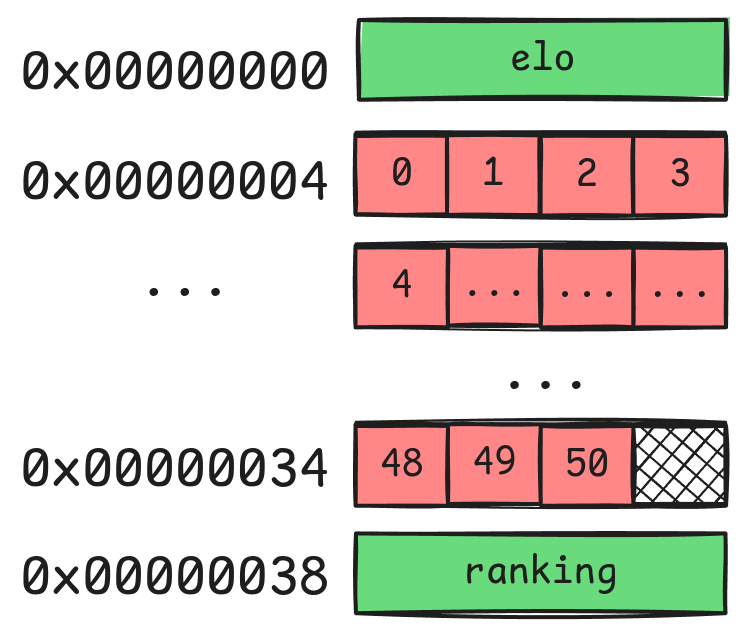
\includegraphics[scale=0.3]{./img/struct.png}  
  \captionof{table}{Struct en memoria}
  \label{fig:struct}
\end{center}

Notar el \textit{padding} que existe entre el array y el campo \hl{ranking}.
Esto se debe a que el compilador alinea los datos en memoria para optimizar el acceso a ellos. En este caso, el compilador decidió alinear el campo \hl{ranking} a un múltiplo de 4 bytes, lo que puede ser útil para mejorar la eficiencia del acceso a la memoria. Veremos en más detalle el tema de alineación y padding en la guia de Assembly. 

Podemos inicializar una estructura al momento de declararla, usando llaves:

\begin{cbox}[]{Inicialización de struct}
#define NAME_LEN 50

struct player{
  int elo;
  char name[NAME_LEN + 1];
  int ranking;
};

struct player player1 = { 2800, "Magnus Carlsen", 1 },
struct player player2 = { 2700, "Fabiano Caruana", 2 };

\end{cbox}

En este momento, es conveniente mencionar el keyword \hl{typedef}, que nos permite definir un nuevo tipo de dato basado en un tipo existente. El nuevo tipo también se conoce por el nombre de \textbf{type alias}. 
Esto es útil para simplificar la declaración de estructuras y hacer el código más legible. 

\begin{cbox}[]{typedef}
typedef float real_t;
typedef int quantity_t;
typedef unsigned long int size_t; // en <stdint.h>
typedef uint32_t vaddr_t; // direccion virtual.
typedef uint32_t paddr_t; // direccion fisica.
\end{cbox}

Notar como primero viene el tipo original y luego el nuevo tipo.

En el siguiente fragmento definimos una estructura y le asignamos un alias \hl{player\_t} para poder usarlo más fácilmente en el resto del código. Además, notar el tipo de inicialización alternativa de \hl{player3}:

\begin{cbox}[]{typedef de struct}
#define NAME_LEN 50

typedef struct {
  int elo;
  char name[NAME_LEN + 1];
  int ranking;
} player_t;

player_t player1 = { 2800, "Magnus Carlsen", 1 },
player_t player2 = { 2700, "Fabiano Caruana", 2 };
player_t player3 = { .name = "Hikaru Nakamura", 
                     .ranking = 3, 
                     .elo = 2600}; //forma alternativa
\end{cbox}

Por otro lado, la operación asignación \hl{=} en \hl{struct} produce una copia de la estructura completa.

\begin{cbox}[]{miembros}
player_t magnus = { 2800, "Magnus Carlsen", 1 },
player_t faustino;

printf("Elo: %d\n", magnus.elo);
printf("Name: %s\n", magnus.name);
printf("Ranking: %d\n", magnus.ranking);

magnus.elo = 2700;
magnus.ranking--;

faustino = magnus; // copia de estructura
\end{cbox}

Las estructuras pueden pasarse a funciones como argumentos y también pueden ser devueltas como valores de retorno.

\begin{cbox}[]{struct como argumento y valor de retorno}

player_t get_player(void) {
  player_t player = { 3000, "Bobby Fischer", 1 };
  return player;
}

void print_player(player_t player) {
  printf("Elo: %d\n", player.elo);
  printf("Name: %s\n", player.name);
  printf("Ranking: %d\n", player.ranking);
}

\end{cbox}

Notar que pasar estructuras grandes de esta manera puede ser ineficiente, ya que se copian todos los datos de la estructura. En su lugar, se suele usar punteros a estructuras, que son más eficientes. Lo veremos más adelante.

Nada impide que armemos un array de estructuras, como el siguiente:

\begin{cbox}[]{array de struct}
typedef struct {
  char* pais;
  int code;
} dials_code_t;

dials_code_t country_codes[] = {
  {"Argentina", 54},
  {"Brasil", 55},
  {"Chile", 56},
  {"Uruguay", 598}
};

printf("Código para Argentina: %d\n", country_codes[0].code);
\end{cbox}

La inicialización puede ser parcial también, como en el siguiente ejemplo:

\begin{cbox}[]{Inicialización de array de struct}
dials_code_t country_codes[100] = {
  [0] = {"Argentina", 54},
  [1] = {"Brasil", 55},
  [2] = {"Chile", 56},
  [3].pais = "Uruguay", [3].code = 598,
  // ... el resto se inicializa en 0
};
\end{cbox}

\begin{exbox}
  Definir una estructura \hl{monstruo\_t} que contenga los siguientes campos:
  \begin{itemize}
    \item \hl{nombre} (string)
    \item \hl{vida} (entero)
    \item \hl{ataque} (double)
    \item \hl{defensa} (double)
  \end{itemize}
  Luego, inicializar un array de monstruos y mostrar por pantalla el nombre y la vida de cada uno de ellos.
\end{exbox}

\begin{exbox}
  Definir una función \hl{evolution} que reciba un \hl{monstruo\_t} y devuelva un nuevo monstruo con los mismos atributos, pero con el ataque y defensa aumentados en 10. Luego, usar esta función para evolucionar un monstruo y mostrar por pantalla sus atributos antes y después de la evolución.
\end{exbox} 

\newpage
\section*{Punteros}

\epigraph{\textit{Paradox is a pointer telling you to look beyond it. If paradoxes bother you, that betrays your deep desire for absolutes. The relativist treats a paradox merely as interesting, perhaps amusing or even, dreadful thought, educational.}}

\subsection*{¿Qué es un puntero?}

\begin{importantbox}
  \centering
  Un puntero es una \textbf{variable que almacena una dirección de memoria}.
\end{importantbox}

\begin{center}
  
\includegraphics[scale=0.1]{./img/lionelhutz-contract.png}  
  \label{fig:simpsons-puntero}
\end{center}

En la guía anterior mencionamos al pasar que uno de los tipos nativos de C es el \textbf{puntero}, tipado \hl{int*}, \hl{char*}, \hl{void*}, etc.
Comencemos mirando el siguiente código:

\begin{cbox}[unbreakable,label=sni:xp,nameref={Snippet \ref{sni:xp}}]{}
  #include <stdio.h>

  int main(){
      int x = 42;
      int *p = &x;
  
      printf("Direccion de x:  %p Valor: %d\n", (void*) &x, x);
      printf("Direccion de p: %p Valor: %p\n", (void*) &p, (void*) p);
      printf("Valor de lo que apunta p: %d\n", *p);
  }
\end{cbox}

\begin{exbox}[label=ejercicio1]
  Sin correr el código, responder:
  \begin{itemize}
    \item ¿Cuál es la diferencia entre \texttt{x} y \texttt{p}? ¿Y entre \texttt{x} y \texttt{\&x}? ¿Y entre \texttt{p} y \texttt{*p}?
    \item ¿Qué valores creen que se van a imprimir por terminal?
  \end{itemize}
\end{exbox}

\begin{exbox}[label=ejercicio2]
  Compilar y ejecutar el código. 
  ¿Qué valores se imprimieron?
  ¿Qué creen que significan?
\end{exbox}

Para responder estas preguntas, es \textbf{clave} que entendamos como se organiza la memoria en C.

Al final del día, la memoria no es más que una tira de \textbf{bits} (1/0).
Pero usualmente queremos trabajar con variables con más valores que solo 0 y 1\footnote{Tener memorias del tamaño que utilizamos hoy, direccionables con granularidad de bit sería caro y dificultoso de implementar a nivel hardware. Este post de quora da una intuición al respecto \url{https://www.quora.com/Why-do-memory-addresses-use-the-unit-of-byte-instead-of-bit}.}, por lo que hoy en día usamos a la memoria como si fuera una tira de \textbf{bytes}, que son grupos de \textbf{8 bits}.

Entonces, desde ahora, pensemos a la memoria como una \textbf{tira de bytes contiguos}.
Vamos a poder acceder a cada uno de estos bytes individualmente, porque cada uno tiene una \textbf{dirección única} que lo identifica.

Llamamos \textbf{puntero} a una variable que guarda la dirección de un valor en memoria. Por ejemplo, si la memoria de la dirección \texttt{0xF0} (hexadecimal) a \texttt{0xF8} tiene esta pinta:
%
\begin{center}
  \noindent \makebox[\textwidth]{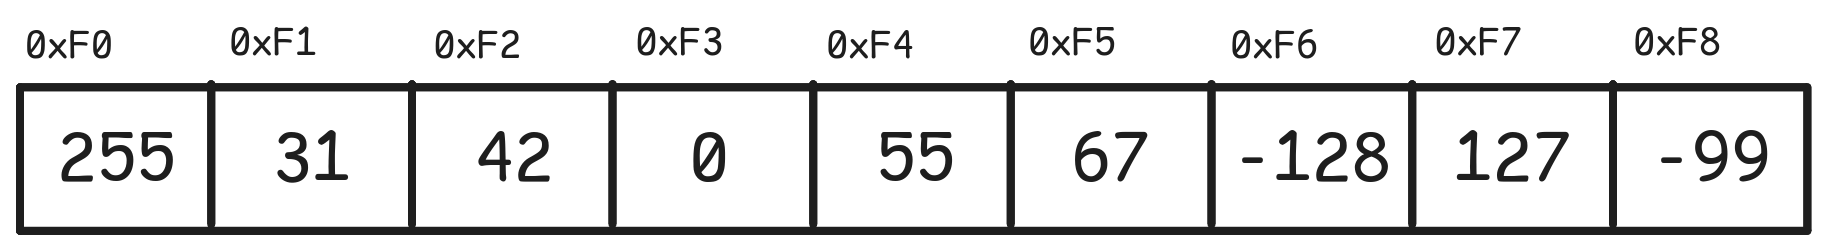
\includegraphics[width=0.5\paperwidth]{./img/memoria_bytes.png}}
  \label{fig:tira-memoria}
\end{center}
%
Podríamos declarar las siguientes variables:
\begin{cbox}[unbreakable]{}
  #include <stdio.h>
  #include <stdint.h>

  int main(){
    uint8_t *x = (uint8_t*) 0xF0;
    int8_t *y = (int8_t*) 0xF6;

    printf("Dir de x: %p Valor: %d\n", (void*) x, *x);
    printf("Dir de y: %p Valor: %d\n", (void*) y, *y);

    //Devolverá:
    //  Dir de x: 0xF0 Valor: 255
    //  Dir de y: 0xF6 Valor: -128
  }
\end{cbox}

\begin{exbox}[label=ejercicio3]
  ¿Por qué \texttt{x} e \texttt{y} tienen distintos tipos? ¿Qué representan?
\end{exbox}

Si intentan ejecutar ese código, probablemente el programa falle con un error de tipo \texttt{Segmentation fault (core dumped)}.
En nuestra computadora, la memoria esta siendo usada por varios componentes y es estadísticamente imposible que las direcciones \texttt{0xF0} a \texttt{0xF8} tengan los valores que usamos en este ejemplo.
De hecho, las direcciones \texttt{0xF0} a \texttt{0xF8} de memoria probablemente no estén a nuestro alcance porque seguramente las esté usando otro proceso (por ende ocurre un \texttt{Segmentation Fault}).

Si queremos una tira contigua de bytes como la mostrada en la imagen, necesitamos declararla.
Para eso, ¡podemos usar arrays! Como vimos en la guía anterior.

\begin{exbox}[label=ejercicio4]
  Completar los ?? en el siguiente código:

  \begin{cbox}[unbreakable]{}
    #include <stdio.h>
    #include <stdint.h>

    int main(){
        int8_t memoria[??] = ??;
        uint8_t *x = (uint8_t*) ??;
        int8_t *y = ??;

        printf("Dir de x: %p Valor: %d\n", (void*) x, *x);
        printf("Dir de y: %p Valor: %d\n", (void*) y, *y);
    }
  \end{cbox}

  \textbf{Pista:} ¿Para qué sirve el operador \texttt{\&}? Revisar los ejemplos de código anteriores o ver la sección \nameref{sec:operadores}.
\end{exbox}

\subsection*{Operando con punteros} 
\label{sec:operadores}

Habrán visto en los ejemplos hasta ahora que al trabajar con punteros contamos con dos operadores principales: \texttt{*} y \texttt{\&}.
Definamos propiamente:

\begin{itemize}
  \item \texttt{*}: se usa en dos situaciones
  \begin{itemize}
    \item Al \textbf{declarar} un puntero: indica que la variable siendo declarada es un puntero al tipo indicado.
    Por ejemplo, \hl{int *num;}\footnote{es equivalente declararlo como \hl{int* num;}. Como era de esperarse, esto lleva a innumerables debates no saldados en internet, por ejemplo: \url{https://stackoverflow.com/questions/398395}} significa que \hl{num} es un puntero a un número entero.
    \item Cuando acompaña a una variable ya declarada: nos permite \textbf{desreferenciar} la variable que acompaña (que debería ser un puntero), permitiéndonos acceder al valor que se encuentra en la dirección guardada en la variable.
    
    Por ejemplo, en el \nameref{sni:xp}, pueden ver que en el último \hl{printf}, donde imprimimos el valor de lo que apunta \hl{p}, para acceder a ese valor usamos \hl{*p}. 
    Efectivamente, ese \hl{printf} resulta en que se imprima \hl{42} a consola.
  \end{itemize}
  \item \texttt{\&}: se usa para obtener la dirección de una variable.
  En el \nameref{sni:xp}, usamos \hl{\&x} para declarar \hl{p} ya que queríamos que el puntero \hl{p} guardara la dirección de la variable \hl{x} (es decir, la dirección donde está guardado el valor 42). 
\end{itemize}

\subsection*{Punteros a punteros}

Hasta ahora solo usamos punteros a valores enteros, pero dado que un puntero no es más que la dirección de memoria de algún valor de algún tipo, podemos tener \textbf{punteros a cualquier cosa}.
¡Incluso podemos tener punteros a punteros!

Algunos ejemplos:
\begin{itemize}
  \item \hl{char*}: puntero a una tira de \hl{char}s. Si su último carácter es un \hl{\textquotesingle\textbackslash0\textquotesingle}, es equivalente a un string.
  \item \hl{int**}: puntero (\texttt{int*\textcolor{red}{*}}) a un puntero a un entero (\texttt{\textcolor{red}{int*}*})
  \item \hl{void*}: puntero a un tipo \textbf{desconocido}.
        No se puede desreferenciar sin antes especificar su tipo mediante un \textbf{casteo}.
\end{itemize}
%
\begin{center}
  \noindent \makebox[\textwidth]{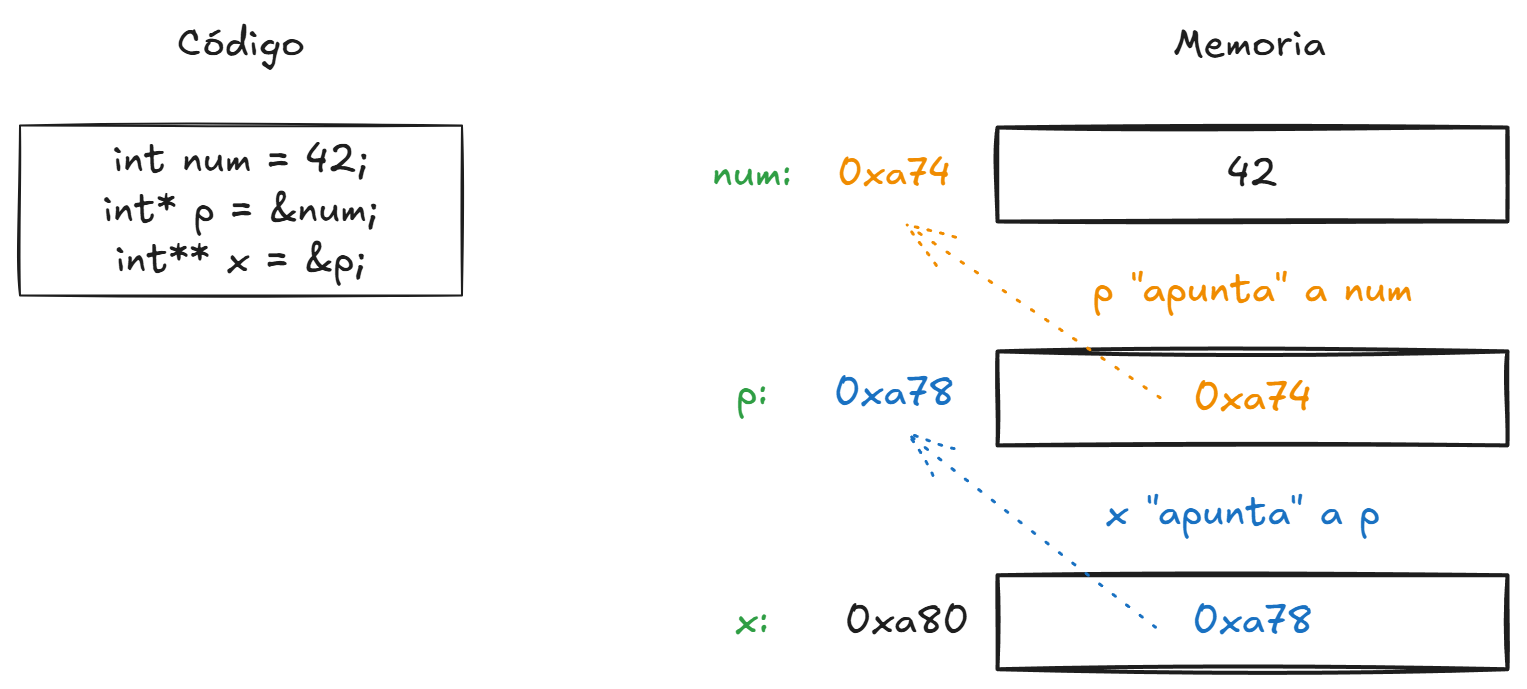
\includegraphics[width=0.7\paperwidth]{./img/puntero y doble puntero.png}}
  \label{fig:doble-puntero}
\end{center}

\subsection*{Castear}

\subsection*{Tipos de memoria}

Tenemos varios tipos de memoria, y en cuál se encuentra nuestra variable dependerá de dónde y cómo declaramos nuestras variables.

\begin{center}
  \begin{table}[!h]
    \centering
    \resizebox{\textwidth}{!}{%
    \begin{tabular}{|c|c|c|}
    \hline
    \rowcolor[HTML]{333333} 
    {\color[HTML]{FFFFFF} \textbf{Tipos de memoria}} & {\color[HTML]{FFFFFF} \textbf{Scope}} & {\color[HTML]{FFFFFF} \textbf{Lifetime}}                                      \\ \hline
    Global                                           & El archivo completo                   & \begin{tabular}[c]{@{}c@{}}el tiempo de vida \\ de la aplicación\end{tabular} \\ \hline
    Estática &
      \begin{tabular}[c]{@{}c@{}}La función (o bloque) \\ donde está declarada\end{tabular} &
      \begin{tabular}[c]{@{}c@{}}el tiempo de vida \\ de la aplicación\end{tabular} \\ \hline
    Automática (local) &
      \begin{tabular}[c]{@{}c@{}}La función (o bloque) \\ donde está declarada\end{tabular} &
      \begin{tabular}[c]{@{}c@{}}Mientras la función (o bloque)\\ esté en ejecución\end{tabular} \\ \hline
    Dinámica &
      \begin{tabular}[c]{@{}c@{}}Determinado por los punteros que\\  referencian esta memoria\end{tabular} &
      \begin{tabular}[c]{@{}c@{}}Hasta que la memoria\\  sea liberada\end{tabular} \\ \hline
    \end{tabular}%
    }
    \end{table}
  
\end{center}
\end{document}
